\section{Алгоритм на основе нисходящего анализа}

GLL~\cite{Grigorev:2017:CPQ:3166094.3166104}

Другие реализации~\cite{MEDEIROS201975}

\subsection{Нисходящий синтаксический анализ}

Рекурсивный спуск, LL, таблицы, неоднозначности, левая рекурсия.

\subsubsection{Рекурсивный спуск}

\subsubsection{LL(k)-алгоритм синтаксического анализа}

LL(k)-алгоритм синтаксического анализа~--- нисходящий анализ без отката, но с предпросмотром.
Решение о том, какую продукцию применять, принимается на основании k следующих за текущим символом.
Временная сложность алгоритма $O(n)$, где $n$~--- длина слова.

Алгоритм использует входной буфер, стек для хранения промежуточных данных и таблицу анализатора, которая управляет процессом разбора.
В ячейке таблицы указано правило, которое нужно применять, если рассматривается нетерминал $A$, а следующий символ строки~--- $t$.
Также в таблице выделена отдельная колонка для $\$$~--- маркера конца строки.

\begin{center}
  \begin{tabular}{ c || c | c | c | c }
             & $\dots$ & t & $\dots$ & $\$$ \\ \hline
    $\dots$  & $\dots$ & $\dots$ & $\dots$ & $\dots$ \\ \hline
    $A$  & $\dots$ & $A \to \alpha$ & $\dots$ & $\dots$ \\ \hline
    $\dots$  & $\dots$ & $\dots$ & $\dots$ & $\dots$
  \end{tabular}
\end{center}

Для построения таблицы вычисляются множества $\first[k]$ и $\follow[k]$.

\begin{definition}
  Пусть $G = \langle N, \Sigma, P, S \rangle$~--- КС-грамматика. Множество $\first[k]$ определено для сентециальной формы $\alpha$ следующим образом:
  \[ \first[k](\alpha) = \{ \omega \in \Sigma^* \mid \alpha \derives{} \omega \text{ и } |\omega| < k \text{ либо } \exists \beta: \alpha \derives{} \omega \beta \text{ и } |\omega| = k \} \text{, где } \alpha, \beta \in (N \cup \Sigma)^* \]
\end{definition}

\begin{definition}
  Пусть $G = \langle N, \Sigma, P, S \rangle$~--- КС-грамматика. Множество $\follow[k]$ определено для сентециальной формы $\beta$ следующим образом:
  \[\follow[k](\beta) = \{ \omega \in \Sigma^* \mid \exists \gamma, \alpha: S \derives{} \gamma \beta \alpha \text{ и } \omega \in \first[k](\alpha) \} \]
\end{definition}

В частном случае для $k = 1$:

\[ \first(\alpha) = \{ a \in \Sigma \mid \exists \gamma \in (N \cup \Sigma)^*: \alpha \derives{} a \gamma \} \text{, где } \alpha \in (N \cup \Sigma)^* \]

\[ \follow(\beta) = \{ a \in \Sigma \mid \exists \gamma, \alpha \in (N \cup \Sigma)^* : S \derives{} \gamma \beta a \alpha \} \text{, где } \beta \in (N \cup \Sigma)^*  \]

Множество $\first$ можно вычислить, пользуясь следующими соотношениями:

\begin{itemize}
  \item $\first(a \alpha) = \{a\}, a \in \Sigma, \alpha \in (N \cup \Sigma)^* $
  \item $\first(\varepsilon) = \{\varepsilon\}$
  \item $\first(\alpha \beta) = \first(\alpha) \cup (\first(\beta) \text{, если } \varepsilon \in \first(\alpha))$
  \item $\first(A) = \first(\alpha) \cup \first(\beta) \text{, если в грамматике есть правило } A \to \alpha \mid\beta$
\end{itemize}

Алгоритм для вычисления множества $\follow$:

\begin{itemize}
  \item Положим $\follow(X) = \varnothing, \forall X \in N$
  \item $\follow(S) = \follow(S) \cup \{\$\} \text{, где } S \text{--- стартовый нетерминал}$
  \item Для всех правил вида $A \to \alpha X \beta: \follow(X) = \follow(X) \cup (\first(\beta) \setminus \{\varepsilon\} )$
  \item Для всех правил вида $A \to \alpha X \text{ и } A \to \alpha X \beta \text{, где } \varepsilon \in \first(\beta): \follow(X) = \follow(X) \cup \follow(A)$
  \item Последние два пункта применяются пока есть что добавлять в строящиеся множества.
\end{itemize}

Пример множеств $\first$ для нетерминалов следующей грамматики:

\begin{multicols}{2}
\begin{align*}
  S  &\to a S' \\
  S' &\to A b B S' \mid \varepsilon \\
  A  &\to a A' \mid \varepsilon \\
  A' &\to b \mid a \\
  B  &\to c \mid \varepsilon
\end{align*}

\columnbreak

\begin{align*}
  \first(S)  &= \{ a \} \\
  \first(A)  &= \{ a, \varepsilon \} \\
  \first(A') &= \{ a, b \} \\
  \first(B)  &= \{ c, \varepsilon \} \\
  \first(S') &= \{ a, b, \varepsilon \}
\end{align*}
\end{multicols}

Пример множеств $\follow$ для нетерминалов следующей грамматики:

\begin{multicols}{2}
\begin{align*}
  S  &\to a S' \\
  S' &\to A b B S' \mid \varepsilon \\
  A  &\to a A' \mid \varepsilon \\
  A' &\to b \mid a \\
  B  &\to c \mid \varepsilon
\end{align*}

\columnbreak

\begin{align*}
  \follow(S)  &= \{ \$ \} & \\
  \follow(S') &= \{ \$ \} &(S \to a S')\\
  \follow(A)  &= \{ b \}  &(S' \to A b B S') \\
  \follow(A') &= \{ b \}  &(A \to a A')\\
  \follow(B)  &= \{ a, b, \$ \} &(S' \to A b B S', \varepsilon \in \first(S'))
\end{align*}
\end{multicols}

Таблица заполняется следующим образом: продукции $A \to \alpha, \alpha \neq \varepsilon$ помещаются в ячейки $(A, a)$, где $a \in \first(A)$, продукции $A \to \varepsilon$~--- в ячейки $(A, a)$, где $a \in \follow(A)$

\begin{example}

Пример таблицы для грамматики $S \to ( S ) \mid \varepsilon$

\begin{center}
\begin{tabular}{ r || c | c || c | c | c }
N & $\first$ & $\follow$ & ( & ) & $\$ $ \\ \hline
$S$ & $\{ (, \varepsilon \}$ & $\{ ), \$ \}$ & $S \rightarrow (S)$ & $S \rightarrow \varepsilon$ & $S \rightarrow \varepsilon$
\end{tabular}
\end{center}

\end{example}

А что, если в ячейку несколько записей? Значит нам не повезло и граммтика неоднозначна. Можно попробовать увеличить $k$. Но и это может не помочь. Когда?

А что будет, если есть леворекурсивные правила?

Интерпретатор автомата принимает входную строку и построенную управляющую таблицу и работает следующим образом.
В каждый момент времени конфигурация автомата это позиция во входной строке и стек.
В начальный момент времени стэк пуст, а позиция во входной строке соответствует её началу.
На певом шаге в стек добавляются последовательно сперва симаол концы строки, затем стартовый нетерминал.
На каждом шаге анализируется существующая конфигурация и совершается одно из действий.
\begin{itemize}
\item Если текущая позиция --- конец строки и вершина стека --- символ конца строки, то успешно завершаем разбор.
\item Если текушая вершина стека --- терминал, то проверяем, что позиция в строке соответствует этому терминалу. Если да, то снимаем элемент со стека, сдвигаем позицию на единицу и продолжаем разбор. Иначе завершаем разбор с ошибкой.
\item Если текущая врешина стека --- нетерминал $N_i$ и текущий входной символ $t_j$, то ищем в управляющей таблице ячейку с координатими $(N_i, t_j)$ и записываем на стек содержимое этой ячейки.
\end{itemize}

\begin{example}Пример работы LL анализатора.
  Таблца вида (стек, указатель во входе, комментарии)
\end{example}

Проблемы с левой рекурсией.

А ещё надо бы деревья научиться строить.

\begin{example}Пример работы LL анализатора с деревом.
  Таблца вида (стек, указатель во входе, дерево, комментарии)
\end{example}

Итого. По некоторым граммтикам можно построить LL(k) анализатор (назовём их LL(k) граммтиками), но не по всем.
С левой рекурсией, конечно, можно бороться, существуют алгоритмы устранения левой и скрытой левой рекурсии, а вот с неодносзначностями ничего не поделаешь.



\subsection{GLL и его применение для КС запросов}

Можно построить анализатор, работающий с произвольными КС-грамматиками.
Generalized LL (GLL)~\cite{Scott:2010:GP:1860132.1860320,10.1007/978-3-662-46663-6_5}

Принцип работы остается абсолютно таким же как и для табличного LL: 
\begin{itemize}
  \item Сначала по грамматике строится \textit{управляющая} таблица
  \item Затем построенная таблица команд и непосредственно анализируемое слово поступают на вход абстрактному интерпретатору.
  \item Для своей работы интерпретатор поддерживает некоторую вспомогательную структуру данных (стек для LL).
  \item Один шаг разбора состоит в том, чтобы рассмотреть текущую позицию в слове, применить соответствующее ей правило из таблицы и при возможности сдвинуть позицию разбора вправо.
\end{itemize}

Где в этой схеме возникают ограничения на вид обрабатываемой грамматики для алгоритма LL? На самом первом шаге --- при построении таблицы может возникнуть ситуация, когда одному нетерминалу $N_j$ и последовательности $first_k(N_j)$ соответствует несколько продукций грамматики. В этом случае грамматика признавалась не соответствующей классу LL(k) и отвергалась анализатором.

Теперь же мы разрешим такую ситуацию и в этом случае в ячейку таблицы будем записывать все продукции грамматики, соответствующие этой ячейке. Однако сразу же возникает вопрос --- а что делать интерпретатору, когда при разборе ему необходимо применить правило, состоящее из нескольких продукций? Общий ответ такой --- необходим некоторый вид недетерминизма, при котором интерпретатор мог бы "параллельно" обрабатывать несколько возможных вариантов синтаксического разбора.

Эти два свойства (модифицированная управляющая таблица и недетерминизм) суть главные принципиальные отличия GLL(k) от LL(k). Далее мы перейдем к рассмотрению непосредственно технической реализации описанного алгоритма.

Нам необходимо научиться задавать различные ветви (пути) синтаксического разбора и переключаться между ними. Заметим, что состояние любой ветви в любой момент времени суть следующее: необходимо распознать символ $N_j \in N \cup \Sigma$ из продукции $X$, начиная с элемента слова под индексом $i$. Т.е. имеем позицию в слове и позицию символа в продукции. Последнее принято называть \textit{слотом грамматики}. 

\begin{definition}
  Пусть $G = \langle N, \Sigma, P, S \rangle$~--- КС-грамматика. \textit{Слотом грамматики} $G$ (позицией грамматики $G$) назовем пару из продукции $X \in P$ и позиции $0 \leq q \leq length(body(X))$ тела продукции $X$. При этом введем следующее обозначение $X ::= \alpha \cdot \beta, \quad \alpha,\beta \in (N \cup \Sigma)^*$, где $ \cdot $ указывает на позицию в продукции.
\end{definition}

Описанная пара позиций уже однозначно задает состояние синтаксического разбора. Имеем множество состояний и переходов между ними --- возникает естественное желание воспользоваться терминами графов для представления этой структуры. Такую конструкцию называют \textit{граф-структурированный стек} или \textit{GSS} (Graph Structured Stack), который впервые был предложен Масару Томитой ~\cite{tomita1988graph} в контексте восходящего анализа. GSS будет являться рабочей структурой нашего нового интерпретатора, вместо стека для LL. Состояние разбора вместе с узлом GSS мы будет называть \textit{дескриптором}.

\begin{definition} 
	Пусть $G = \langle N, \Sigma, P, S \rangle$~--- КС-грамматика, $X$ слот грамматики $G$, $i$ позиция в слове $ w $ над алфавитом $\Sigma$, а $ u $ узел GSS. \textit{Дескриптором} назовём тройку $ (X, u, i) $.
\end{definition}

Есть несколько способов задания GSS для алгоритма GLL. Вариант, предложенный самими авторами алгоритма, оперирует непосредственно парами из позиции слова и слота грамматики в качестве состояний (и узлов графа) --- такой метод является довольно простым и наглядным, но, как описано в работе \cite{10.1007/978-3-662-46663-6_5}, не самым эффективным. Предложим сразу чуть более оптимальное представление: заметим, что шаги разбора, соответствующие одному и тому же нетерминалу и позиции слова, должны выдавать один и тот же результат независимо от конкретной продукции грамматики, в которой стоит этот нетерминал. Поэтому заводить по узлу на каждый слот грамматики довольно избыточно --- вместо этого в качестве состояния будет использовать пары из нетерминала и позиции слова, а позиции грамматики будем записывать на рёбрах.  

Итак, мы научились задавать состояния с помощью дескрипторов, а также определились со вспомогательной структурой GSS. Теперь можно перейти к рассмотрению непосредственно самого алгоритма, суть которого довольно проста и напоминает BFS по неявному графу.

Дескриптор задает состояние, которое необходимо обработать. При этом мы без какой-либо дополнительной информации можем продолжить анализ входа из состояния, задаваемого этим дескриптором. В процессе обработки мы можем получить несколько новых состояний. Поэтому будем поддерживать множество $ R $ дескрипторов на обработку --- на каждом шаге извлекаем один из множества, проводим анализ и кладем в множество новые полученные. 

При каких условиях этот процесс будет конечен? Ну, например, если мы каждое состояние будем обрабатывать не более одного раза. И действительно, поскольку наш интерпретатор является ``чистым'' в том смысле, что для оного и того же состояния каждый раз будут получены одинаковые результаты, проводить анализ дважды не имеет смысла. Поэтому будем также поддерживать множество $ U $ всех полученных в ходе разбора дескрипторов, и добавлять в $ R $ только те, которых еще нет в $ U $.

И наконец, заключительная и самая главная часть --- как происходит обработка дескриптора?
Пусть дескриптор имеет вид $ (X, u, i) $, а входное слово обозначим $ W $. Есть три возможных варианта, в зависимости от вида позиции грамматики $ X $ --- разберем каждый из них по отдельности; 

\begin{itemize}
  \item $ X ::= \alpha \cdot t \beta $, т.е. указатель смотрит на терминал --- в этом случае новых дескрипторов добавлено не будет. Если $ W[i] = t $, то мы сдвигаем указатель слота, переходя к рассмотрению $ X ::= \alpha t \cdot \beta $, и инкрементируем позицию $ i $ в слове. В противном же случае сразу переходим к следующему дескриптору, т.о. терминируя текущую ветвь разбора.
  
  \item $ X ::= \alpha \cdot A \beta $, т.е. указатель смотрит на нетерминал. Нам нужен GSS узел $ v $ вида $ (A, i) $ и ребро $ (u, X ::= \alpha A \cdot \beta, v) $ (ребро из $ u $ в $ v $ с пометкой $ X ::= \alpha A \cdot \beta $). Если такой узел и ребро уже существуют в нашем GSS, берем их, иначе --- создаём. Далее в $ R $ добавляем по дескриптору для узла $ v $ и каждого правила грамматики из ячейки управляющей таблицы для нетерминала $ A $ (конечно, если их еще не было в $ U $). На этом обработка текущего дескриптора завершается.
  
  \item $ X ::= \alpha \cdot $, т.е. указатель находится в конце продукции. Продукция разобрана, а значит, интерпретатору необходимо вернуться из разбора $ X $ к вызывающему правилу и продолжить разбор там (это, в некотором смысле, соответствует возврату из функции разбора нетерминала в методе рекурсивного спуска). По каждому исходящему ребру $ (u, Y, v) $ добавляем (если уже не существует) дескриптор $(Y, v, i)$. 
\end{itemize}

Результатом синтаксического разбора является успех тогда и только тогда, когда был достигнут дескриптор вида $ (S ::= \alpha \cdot, s, n) $, где слот грамматики представляет собой любое правило для аксиомы $ S $, узел GSS $ s $ состоит из аксиомы $ S $ и 0, а позиция входного слова равна его длине $ n $. Если же после разбора всех полученных дескрипторов указанный найден не был, результатом будет являться провал.

Давайте посмотрим, как такой алгоритм справится с неоднозачной грамматикой с леворекурсивным правилом. 

\begin{example}

	Пусть грамматика $ G $ имеет вид $ S \to SSS \mid SS \mid a $, а разбираемое слово $ w = aaa $. Тогда GSS, соответствующий разбору $S \Rightarrow SSS \Rightarrow aSS \Rightarrow aaS \Rightarrow aaa$, будет выглядеть следующим образом (для удобства каждое ребро дополнительно пронумеровано):

\begin{center}             

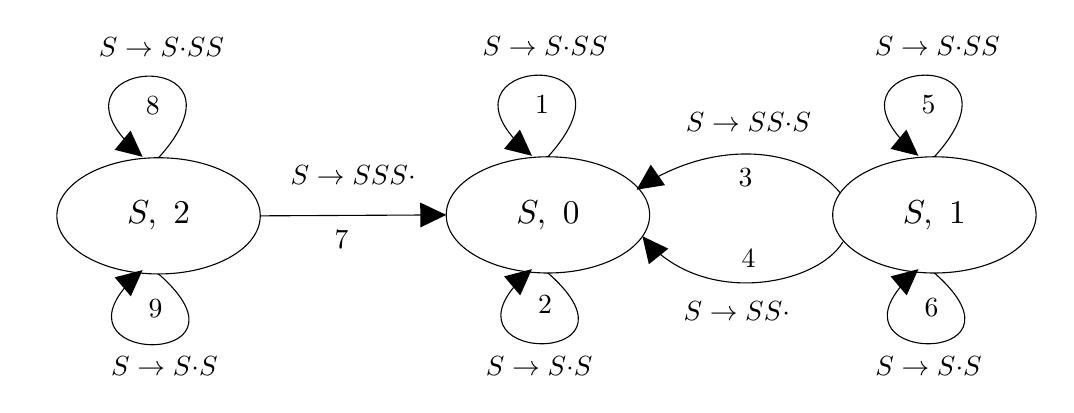
\begin{tikzpicture}[x=0.75pt,y=0.75pt,yscale=-1,xscale=1,scale=1.4]
%uncomment if require: \path (0,300); %set diagram left start at 0, and has height of 300

%Shape: Ellipse [id:dp5003717192946906] 
\draw   (246,139) .. controls (246,127.95) and (261.67,119) .. (281,119) .. controls (300.33,119) and (316,127.95) .. (316,139) .. controls (316,150.05) and (300.33,159) .. (281,159) .. controls (261.67,159) and (246,150.05) .. (246,139) -- cycle ;
%Curve Lines [id:da4659605386988417] 
\draw    (281,119) .. controls (317.14,79.07) and (236.15,84.55) .. (274.31,117.66) ;
\draw [shift={(275.5,118.67)}, rotate = 219.67000000000002] [fill={rgb, 255:red, 0; green, 0; blue, 0 }  ][line width=0.75]  [draw opacity=0] (8.93,-4.29) -- (0,0) -- (8.93,4.29) -- cycle    ;

%Curve Lines [id:da8752346012662928] 
\draw    (281,159) .. controls (319.12,192.33) and (238.15,190.7) .. (274.37,158.65) ;
\draw [shift={(275.5,157.67)}, rotate = 499.76] [fill={rgb, 255:red, 0; green, 0; blue, 0 }  ][line width=0.75]  [draw opacity=0] (8.93,-4.29) -- (0,0) -- (8.93,4.29) -- cycle    ;

%Shape: Ellipse [id:dp8131879975151008] 
\draw   (379,139) .. controls (379,127.95) and (394.67,119) .. (414,119) .. controls (433.33,119) and (449,127.95) .. (449,139) .. controls (449,150.05) and (433.33,159) .. (414,159) .. controls (394.67,159) and (379,150.05) .. (379,139) -- cycle ;
%Curve Lines [id:da5133930309497914] 
\draw    (414,119) .. controls (450.14,79.07) and (369.15,84.55) .. (407.31,117.66) ;
\draw [shift={(408.5,118.67)}, rotate = 219.67000000000002] [fill={rgb, 255:red, 0; green, 0; blue, 0 }  ][line width=0.75]  [draw opacity=0] (8.93,-4.29) -- (0,0) -- (8.93,4.29) -- cycle    ;

%Curve Lines [id:da6453313783075103] 
\draw    (414,159) .. controls (452.12,192.33) and (371.15,190.7) .. (407.37,158.65) ;
\draw [shift={(408.5,157.67)}, rotate = 499.76] [fill={rgb, 255:red, 0; green, 0; blue, 0 }  ][line width=0.75]  [draw opacity=0] (8.93,-4.29) -- (0,0) -- (8.93,4.29) -- cycle    ;

%Curve Lines [id:da37225339830095105] 
\draw    (381.5,131.33) .. controls (368.76,115.65) and (338.73,112.46) .. (313.07,129.28) ;
\draw [shift={(311.5,130.33)}, rotate = 325.3] [fill={rgb, 255:red, 0; green, 0; blue, 0 }  ][line width=0.75]  [draw opacity=0] (8.93,-4.29) -- (0,0) -- (8.93,4.29) -- cycle    ;

%Curve Lines [id:da8745073266278207] 
\draw    (382.5,148.33) .. controls (373.68,163.03) and (335.09,171.01) .. (314.72,147.79) ;
\draw [shift={(313.5,146.33)}, rotate = 411.34000000000003] [fill={rgb, 255:red, 0; green, 0; blue, 0 }  ][line width=0.75]  [draw opacity=0] (8.93,-4.29) -- (0,0) -- (8.93,4.29) -- cycle    ;

%Shape: Ellipse [id:dp1740838291000104] 
\draw   (112,139.33) .. controls (112,128.29) and (127.67,119.33) .. (147,119.33) .. controls (166.33,119.33) and (182,128.29) .. (182,139.33) .. controls (182,150.38) and (166.33,159.33) .. (147,159.33) .. controls (127.67,159.33) and (112,150.38) .. (112,139.33) -- cycle ;
%Curve Lines [id:da09054970105752425] 
\draw    (147,119.33) .. controls (183.14,79.4) and (102.15,84.88) .. (140.31,117.99) ;
\draw [shift={(141.5,119)}, rotate = 219.67000000000002] [fill={rgb, 255:red, 0; green, 0; blue, 0 }  ][line width=0.75]  [draw opacity=0] (8.93,-4.29) -- (0,0) -- (8.93,4.29) -- cycle    ;

%Curve Lines [id:da9843249024164302] 
\draw    (147,159.33) .. controls (185.12,192.66) and (104.15,191.04) .. (140.37,158.98) ;
\draw [shift={(141.5,158)}, rotate = 499.76] [fill={rgb, 255:red, 0; green, 0; blue, 0 }  ][line width=0.75]  [draw opacity=0] (8.93,-4.29) -- (0,0) -- (8.93,4.29) -- cycle    ;

%Straight Lines [id:da5967272370226813] 
\draw    (182,139.33) -- (244,139.01) ;
\draw [shift={(246,139)}, rotate = 539.7] [fill={rgb, 255:red, 0; green, 0; blue, 0 }  ][line width=0.75]  [draw opacity=0] (8.93,-4.29) -- (0,0) -- (8.93,4.29) -- cycle    ;


% Text Node
\draw (281,139) node [scale=1.2]  {$S,\ 0$};
% Text Node
\draw (414,139) node [scale=1.2]  {$S,\ 1$};
% Text Node
\draw (350,107) node {$S \rightarrow SS\mathbf{\cdot } S$};
% Text Node
\draw (346,172) node {$S \rightarrow SS\mathbf{\cdot }$};
% Text Node
\draw (280,81) node {$S \rightarrow S\mathbf{\cdot } SS$};
% Text Node
\draw (415,81) node {$S \rightarrow S\mathbf{\cdot } SS$};
% Text Node
\draw (278,191) node{$S \rightarrow S\mathbf{\cdot } S$};
% Text Node
\draw (412,191) node {$S \rightarrow S\mathbf{\cdot } S$};
% Text Node
\draw (279,101) node {$1$};
% Text Node
\draw (280,170) node {$2$};
% Text Node
\draw (349,126) node {$3$};
% Text Node
\draw (350,154) node {$4$};
% Text Node
\draw (412,101) node {$5$};
% Text Node
\draw (413,171) node {$6$};
% Text Node
\draw (147,139.33) node [scale=1.2] {$S,\ 2$};
% Text Node
\draw (214,125.33) node {$S \rightarrow SSS\mathbf{\cdot }$};
% Text Node
\draw (148,81.33) node {$S \rightarrow S\mathbf{\cdot } SS$};
% Text Node
\draw (145,101.33) node {$8$};
% Text Node
\draw (146,171.33) node {$9$};
% Text Node
\draw (210,147.33) node {$7$};
% Text Node
\draw (149,191) node {$S \rightarrow S\mathbf{\cdot } S$};

\end{tikzpicture}
\end{center}

	Сразу отметим несколько особенностей:
	
	\begin{itemize}
	  \item Это \textit{неполный} GSS. Для задачи синтаксического анализа такого достаточно, поскольку если в какой-то момент был достигнут финальный дескриптор, то обрабатывать все последующие уже не нужно. Однако, для задачи построения SPPF, как мы отметим далее, это уже не так, поскольку она требует агрегирования всех возможных путей разбора.
	
	  \item Обратите особое внимание на наличие петель. Они как раз-таки и обеспечивают эффективную работу с леворекурсивными правилами, поскольку переиспользуются уже существующие узлы. При этом кратных петель, понятно, не создается, т.к. мы запоминаем все достигнутые дескрипторы в множестве $ U $ и дублирующих дескрипторов в рабочее множество $ R $ не добавляем. 
	
    \item В GSS не создаются узлы, соответствующие разбору терминалов (например, $a, 0$). В действительности так можно было бы сделать. Но тогда при обработке слота, указывающего на терминал, сначала бы создался узел GSS, затем интерпретатор сверил бы терминал и символ в слове, после чего, если они совпали, произошел бы возврат из узла, а если нет, узел был бы отброшен и интерпретатор перешел бы к другому дескриптору. Таким образом, при любом случае сначала создается узел, затем выполняется проверка, после чего узел сразу отбрасывается. Для того, чтобы не создавать такие ``одноразовые'' узлы, проверка терминалов выполняется in-place.
	\end{itemize}
  
  Пронумеруем продукции и выпишем управляющую таблицу: 

	\begin{table}[!htb]
	    \begin{minipage}{.5\linewidth}
	      \centering
	      \begin{tabular}{lc}
	          $S \to S S S$ & (0) \\
	          $S \to S S$   & (1) \\ 
	          $S \to a$     & (2)
	      \end{tabular}
	    \end{minipage}%
	    \begin{minipage}{.5\linewidth}
	      \centering
	      \begin{tabular}{ r || c || c | c}
	          N   & $\first$  & a     & $\$ $ \\ \hline
	          $S$ & $\{ a \}$ & 0,1,2 &
	      \end{tabular}
	    \end{minipage} 
	\end{table}

	Разумеется, что конкретный порядок исполнения алгоритма будет зависеть, например, от используемой в качестве рабочего множества $ R $ структуры данных и от порядка обработки правил из ячейки управляющей таблицы. Рассмотрим лишь один из возможных вариантов:
  
  \begin{enumerate}
		\item Для начала мы создаем узел GSS $ s_0 = (S, 0) $ и дескрипторы для правил из ячейки таблицы $ S, a $: $ (S \to \cdot SSS, s_0, 0), (S \to \cdot SS, s_0, 0), (S \to \cdot a, s_0, 0) $. 
     
		\item При обработке $ (S \to \cdot S S S, s_0, 0) $ образовываются петля 1 и дескрипторы \linebreak $ (S \to \cdot SSS, s_0, 0), (S \to \cdot SS, s_0, 0), (S \to \cdot a, s_0, 0) $, которые уже содержатся в множестве $ U $ после шага 1 и поэтому не добавляются повторно. 
     
		\item При обработке $ (S \to \cdot S S, s_0, 0) $ образовывается петля 2, а в остальном аналогично \mbox{шагу 2.}
     
		\item При обработке $ (S \to \cdot a, s_0, 0) $ мы распознаем терминал $a$ на позиции 0 и, возвращаясь по петлям 1 и 2, добавляем дескрипторы $ (S \to S \cdot S S, s_0, 1), (S \to S \cdot S, s_0, 1) $.
    
    \item При обработке $ (S \to S \cdot S S, s_0, 1) $ образовываем узел $s_1 = (S, 1)$ с исходящим ребром 3 и добавляем дескрипторы $ (S \to \cdot SSS, s_1, 1), (S \to \cdot SS, s_1, 1), (S \to \cdot a, s_1, 1) $.
    
    \item При обработке $ (S \to S \cdot S, s_0, 1) $ образовываем ребро 4, новых дескрипторов не добавляется.   
     
		\item Обработка дескриптора $ (S \to \cdot S S S, s_1, 1) $ аналогична шагу 2 с добавлением петли 5.
		
		\item Обработка дескриптора $ (S \to \cdot S S, s_1, 1) $ аналогична шагу 3 с добавлением петли 6.
		
		\item При обработке $ (S \to \cdot a, s_1, 1) $ мы распознаем терминал $a$ на позиции 1 и, возвращаясь по ребрам 3 и 4, добавляем дескрипторы $ (S \to S S \cdot S, s_0, 2), (S \to S S \cdot, s_0, 2) $, а также, возвращаясь по петлям 5 и 6, добавляем дескрипторы $ (S \to S \cdot S S, s_1, 2), (S \to S \cdot S, s_1, 2) $.
		
		\item При обработке $ (S \to S S \cdot S, s_0, 2) $ образовываем узел $s_2 = (S, 2)$ с исходящим ребром 7 и добавляем дескрипторы $ (S \to \cdot SSS, s_2, 2), (S \to \cdot SS, s_2, 2), (S \to \cdot a, s_2, 2) $.
		
		\item Обработка дескриптора $ (S \to \cdot S S S, s_2, 2) $ аналогична шагу 2 с добавлением петли 8.
				
		\item Обработка дескриптора $ (S \to \cdot S S, s_2, 2) $ аналогична шагу 3 с добавлением петли 9.
		
		\item При обработке $ (S \to \cdot a, s_2, 2) $ мы распознаем терминал $a$ на позиции 2 и, возвращаясь по ребру 7, добавляем дескриптор $ (S \to S S S \cdot, s_0, 3) $, а также, возвращаясь по петлям 8 и 9, добавляем дескрипторы $ (S \to S \cdot S S, s_2, 3), (S \to S \cdot S, s_2, 3) $.
		
		\item Мы достигли финального дескриптора $ (S \to S S S \cdot, s_0, 3) $, синтаксический разбор успешен.
  \end{enumerate}

\end{example}

Внимательный читатель мог заметить, что если бы в этом примере шаг 4 был выполнен перед шагом 2, разбор бы довольно быстро завершился неудачей. Отсюда вытекает следующее наблюдение: если в какой-то момент из существующего узла появилось новое ребро, необходимо пересчитать все входящие в него пути. 

Теперь рассмотрим задачу построения SPPF. Конкретные технические реализации будут отличаться в зависимости от типа рассматриваемого SPPF --- одна из наиболее эффективных представлена в работе \cite{10.1007/978-3-662-46663-6_5}. Мы рассмотрим чуть более простую версию, без бинарного сжатия.

\textbf{TODO}

Ну а теперь всё это на граф~\cite{Grigorev:2017:CPQ:3166094.3166104}
Заметим, что позиции всё так же вершины графа.
Дальше всё само собой.

\begin{example} GLL на графе с SPPF.
\end{example}


Детали реализации: иногда лучше не очередь дескрипторов, а стек, так как выше локальность данных --- мы кладём пачку дескрипторов, соответствующих исходящим рёбрам. Зависит от структуры представления графа, но если это список смежности, что исходящие хранятся рядом и их лучше обработать сразу.

\subsection{Вопросы и задачи}
\begin{enumerate}
  \item Проведите алгоритм GLL для примера (вставить ссылку). Пронаблюдайте, как использование GSS вырождается в обыкновенную работу со стеком. 
  \item Доразберите все нерассмотренные в примере (вставить ссылку) дескрипторы, постройте полный GSS.
\end{enumerate}
